% \section{Background}
The ALICE (A Large Ion Collider Experiment) detector is a detector experiment at the Large Hadron Collider (LHC) at CERN. Its primary goal is the investigation of ``strongly interacting matter at extreme energy densities, where a formation of a new phase of matter, the quark-gluon plasma, is expected''~\cite{ALICE_LOI}. It achieves this goal by studying the products of head-on collisions of heavy ions such as lead, called Pb-Pb collisions for short. It also studies proton-lead (p-Pb) and proton-proton (p-p) collisions.  

\subsection{Coordinates}
The coordinate system used at ALICE needs to be discussed in order to fully explain the scope of this report. A modified cylindrical coordinate system, shown in \cref{fig:coords}, is used as most detectors in the experiment are cylindrically symmetric about the beamline of the LHC. 

\begin{figure}[h]
    \begin{center}
        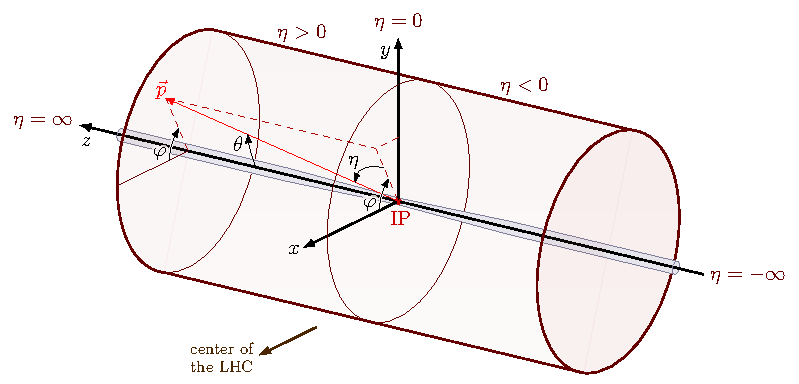
\includegraphics[width=.8\textwidth]{Figs/coords.pdf}
        \caption{Modified cylindrical coordinate system used at the LHC~\cite{coords}.}
        \label{fig:coords}
    \end{center}
\end{figure}

We place the $z$-axis along the beamline with its origin at the interaction point (IP). The IP is the point at which collisions happen, right in the center of the detector. The angle around the $z$-axis is called the azimuthal angle, denoted by $\varphi$. Sometimes in the literature $\varphi$ ranges from 0 to $2\pi$ and sometimes it ranges from $-\pi$ to $\pi$. We will try stay consistent and use the latter in this report, but we may need use the other convention at times. The angle from the $z$-axis to the $x$-$y$ plane is called the polar angle, denoted by $\theta$, and runs from 0 to $\pi$. We are interested in the standard 3-momentum of particles that we track in the detector, which we call $\vec{p}=(p_x,p_y,p_z)$, but we also define the transverse momentum as 
\begin{equation}
    p_{\mathrm{T}}=\sqrt{p_x^2 + p_y^2}.
    \label{eqn:transverse momentum}
\end{equation}
We define the rapidity, often denoted as $y$, as
\begin{equation}
    y=\frac 12 \ln\left(\frac{E+p_z}{E-p_z}\right)
    \label{eqn:rapidity}
\end{equation}
where $E$ is the total energy of the particle being considered and $p_z$ is the momentum in the $z$ direction~\cite{kar_exp_phys}. This quantity is useful as differences in rapidity are Lorentz invariant for boosts along the $z$-axis. One issue, however, is that the energy of a particle is hard to measure, so we instead use pseudorapidity, denoted as $\eta$. Rapidity and pseudorapidity are equivalent for massless particles, and near equivalent for particles with total 3-momentum magnitude $p$ much greater than their mass $m$. Pseudorapidity is much easier to measure as it is defined in \cite{kar_exp_phys} as
\begin{equation}
    \eta=-\ln\tan\frac{\theta}{2}.
    \label{eqn:pseudorapidity}
\end{equation}
From \cref{fig:coords} we see that for $z$ positive, $\eta$ is also positive, and similarly for $z$ negative. Confusingly, we define the ``forward region'' of the ALICE detector as the region for which $z$, and thus $\eta$, are negative. The forward region is where our interest lies.

\subsection{ALICE Run 3}
In 2018, the LHC shut down for what was called Long Shutdown 2 (LS2). During this time, the ALICE experiment was being prepared for Run 3, where it will be taking data at much higher rates and much higher energies than before, from 2022 until 2025~\cite{ALICE_Upgrade_LOI}. \Cref{fig:ALICE_Schematic} shows the detector configuration for Run 3. The intent of these upgrades was in large part to prepare ALICE for a higher frequency of collisions in both Pb-Pb and p-p cases. 

Part of the upgrades for Run 3, the details of which can be found in \cite{ALICE_Upgrade_LOI}, were a whole new Inner Tracking System and a brand new detector called the Muon Forward Tracker. These detectors are both silicon-based and their primary purpose is tracking particles and determining the collision vertex, which is the best estimation of where the collision that resulted in these particles happened. 

The readout electronics for many detectors were also upgraded to allow for continuous readout as opposed to triggered readout. The MCH also had its readout and front-end electronics upgraded but will still work on a triggered readout system.

\subsection{The Inner Tracking System}
The Inner Tracking System (ITS) sits in the main barrel of ALICE, as seen in \cref{fig:ALICE_Schematic}, and covers the range $|\eta|<1.22$~\cite{ITS_Upgrade_TDR}. For Run 3 it has been upgraded significantly by replacing the old detector with a new layout and new detection technology, leading to an improvement in track position resolution at the primary vertex of a factor of 3 or greater~\cite{ITS_Upgrade_TDR}. The ITS's main purpose is to track the particles resulting from the collisions and determine the position of the primary vertex of collisions. It also serves to ``reconstruct secondary vertices, track and identify particles with low momentum, and improve the momentum and angle resolution for particles reconstructed by the Time Projection Chamber (TPC)''~\cite{ITS_Info}.

\begin{figure}[H]
    \begin{center}
        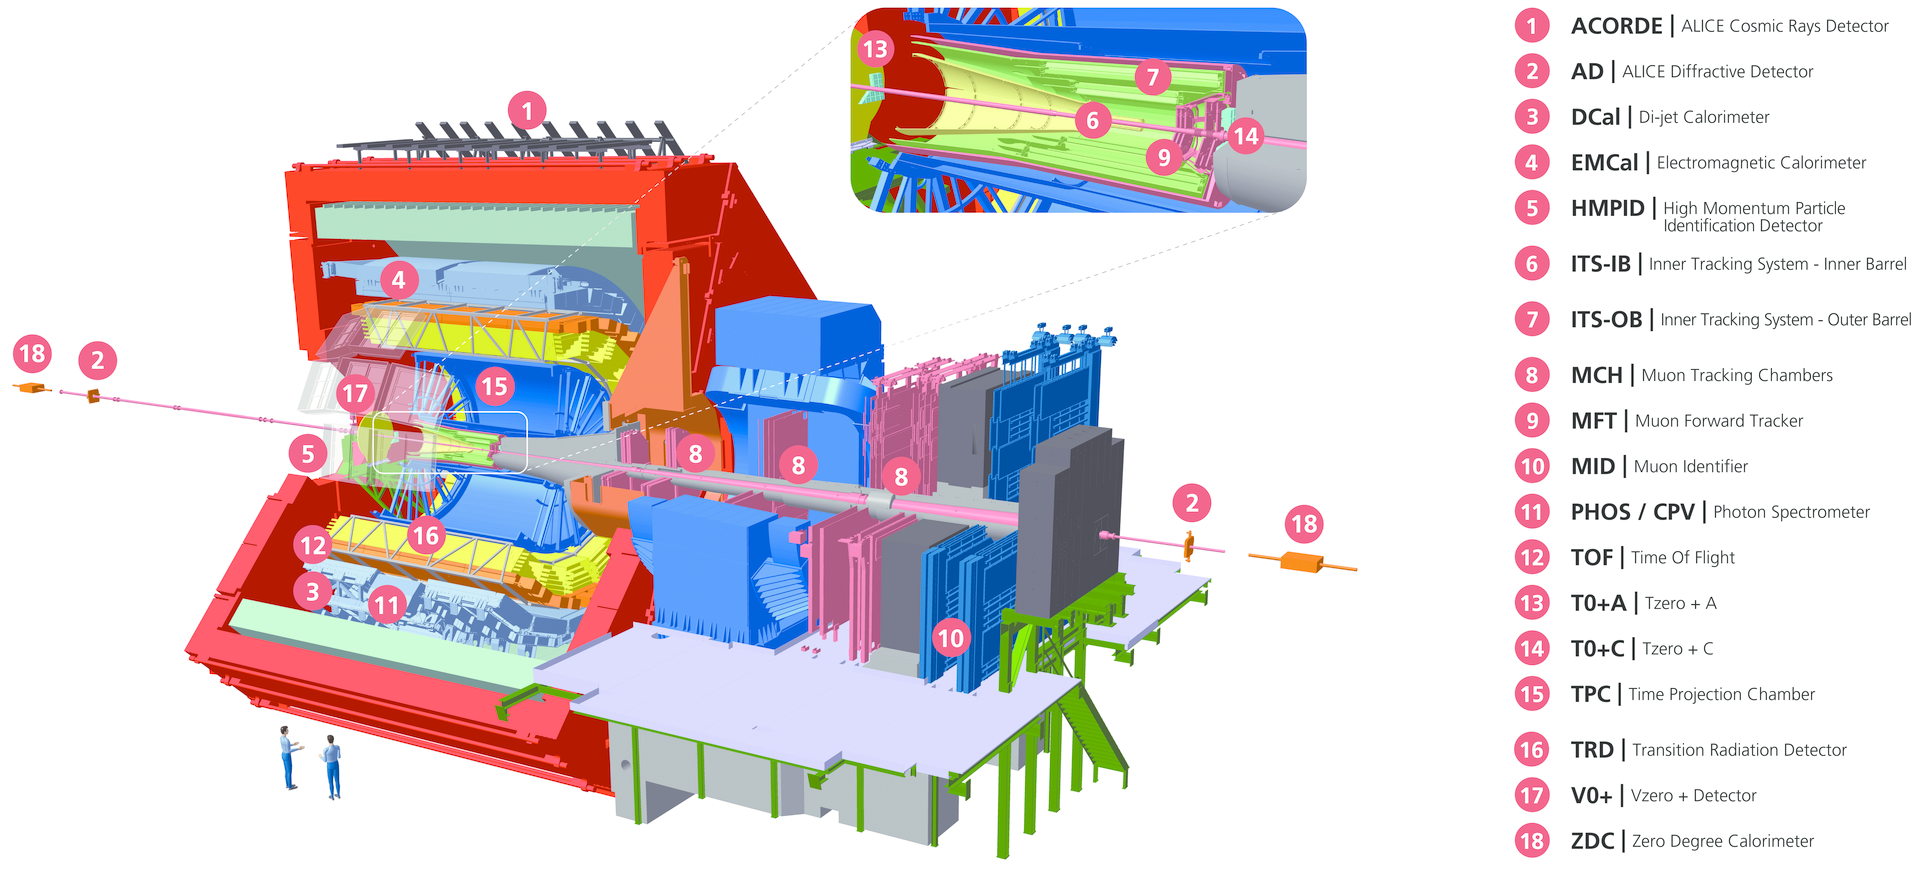
\includegraphics[width=\textwidth]{Figs/ALICE_RUN3_schematic.png}
        \caption{Schematic view of the ALICE detector setup for Run 3 of the LHC~\cite{ALICE_schematic_labels}. Note here that the MCH is shown separate from the MID, which act as the triggering mechanism for the MCH. For the purposes of this report, the MID will be considered part of the MCH.}
        \label{fig:ALICE_Schematic}
    \end{center}
\end{figure}

\begin{figure}[H]
    \begin{center}
        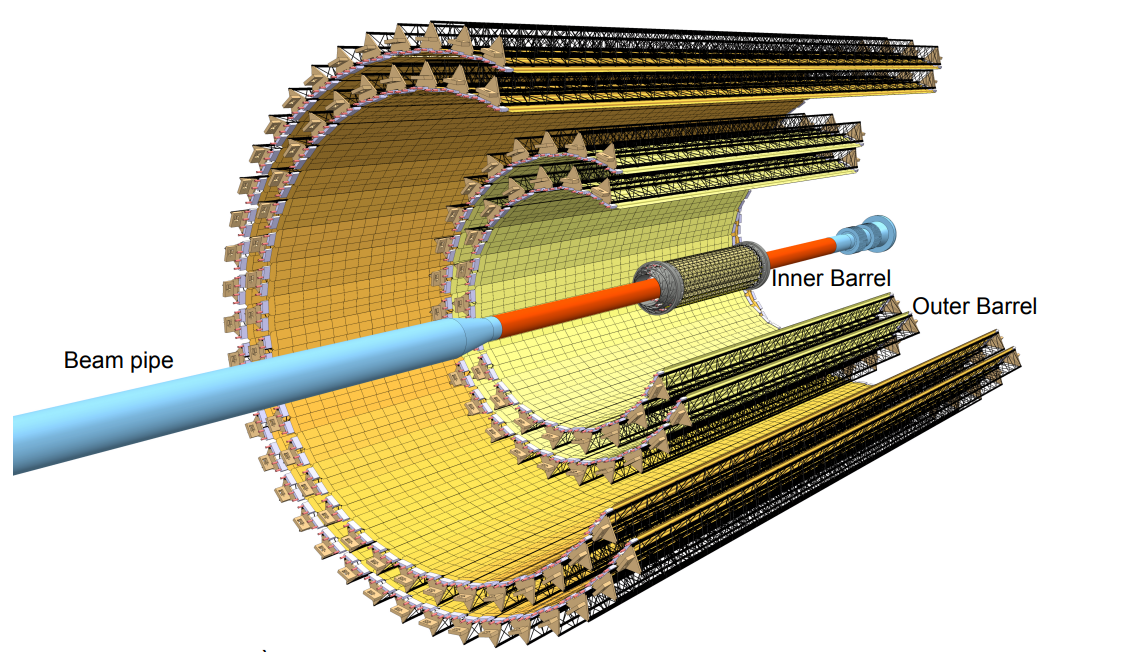
\includegraphics[width=.8\textwidth]{Figs/ITS_Schematic.png}
        \caption{Schematic view of the Inner Tracking System~\cite{ITS_Upgrade_TDR}. Note the thinner beam pipe and extremely close Inner Barrel.}
        \label{fig:ITS_Schematic}
    \end{center}
\end{figure}

The new ITS consists of 7 layers of pixel detectors; 3 in the ``Inner Barrel'' and 4 in the ``Outer Barrel''. The pixel detectors used are \SI{0.18}{\micro\metre} CMOS chips from TowerJazz. When a charged particle passes through the silicon in the active volume, it liberates the charge carriers in the material, which then collect on electrodes connected to the silicon, telling the detector that a particle has been detected. The fine segmentation of the detectors also allows the detector to determine the point at which the particle hit the detector, up to a resolution of \SI{4}{\micro\metre} in both the $r\varphi$ and $z$ directions~\cite{ITS_Upgrade_TDR}.

The innermost layer sits at a radius of only \SI{22.4}{\milli\metre} from the IP thanks to a reduction in beam pipe radius for Run 3 and the outermost layer sits at a radius of \SI{391.8}{\milli\metre} from the IP. \Cref{fig:ITS_Schematic} shows the layout more clearly. 

\subsection{The Muon Spectrometer}
The MCH sits in the forward region of ALICE, as seen in \cref{fig:ALICE_Schematic}, and covers $-4<\eta<-2.5$. It is designed to study heavy quark resonances through their single- and di-muon decay channels.

As is shown in \cref{fig:Muon Spectrometer}, it is composed of a hadronic absorber, tracking chambers, a dipole magnet, and finally the trigger chambers. The MFT is often also considered part of the MCH but is not shown in \cref{fig:Muon Spectrometer}. The absorber, made of carbon and concrete, serves to filter out all particles travelling towards the MCH that are not muons as muons interact very rarely with matter. The 5 tracking chambers track the path of the muons before, during, and after they are bent by the dipole magnet. These tracking chambers used to also do the job of the MFT in Run 1 and Run 2, but with the increase in luminosity and energy of the LHC in Run 3, the MFT needed to be added in order to improve the vertexing capabilities. Lastly, the trigger system consists of two large gas chamber detectors which trigger the MCH to take data only when a muon is detected.

\begin{figure}[h]
    \begin{center}
        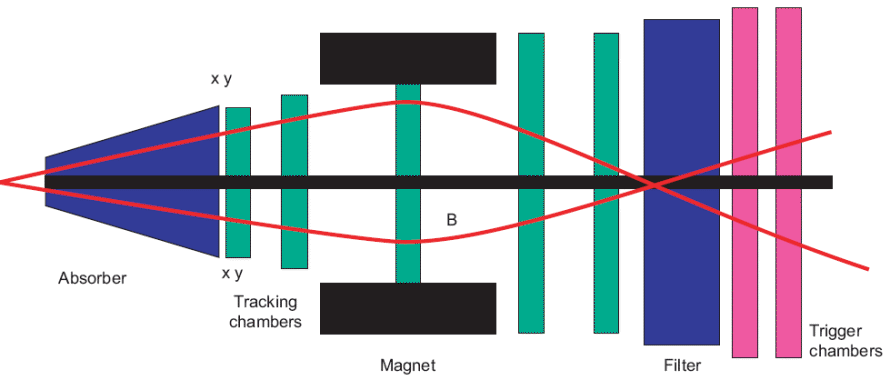
\includegraphics[width=\textwidth]{Figs/MCH_schematic.png}
        \caption{Diagram of the layout of the Muon Spectrometer~\cite{Muon_Spec_Schematic}. Shown in red is an example of the paths of two muons created in a di-muon event.}
        \label{fig:Muon Spectrometer}
    \end{center}
\end{figure}

\subsection{The Muon Forward Tracker}
The MFT is a brand new detector added to ALICE for Run 3. It serves as a tracking detector for the MCH and covers the range $-3.6<\eta<-2.45$. The MFT was made in conjunction with the ITS and uses precisely the same CMOS pixel sensors but in a conical configuration to better suit the geometry of the problem. Due to the MFT being placed in front of the absorber, it detects a lot more particles than make it through to the MCH, allowing it to be much better at finding the primary vertex of collisions.

\begin{figure}[h]
    \begin{center}
        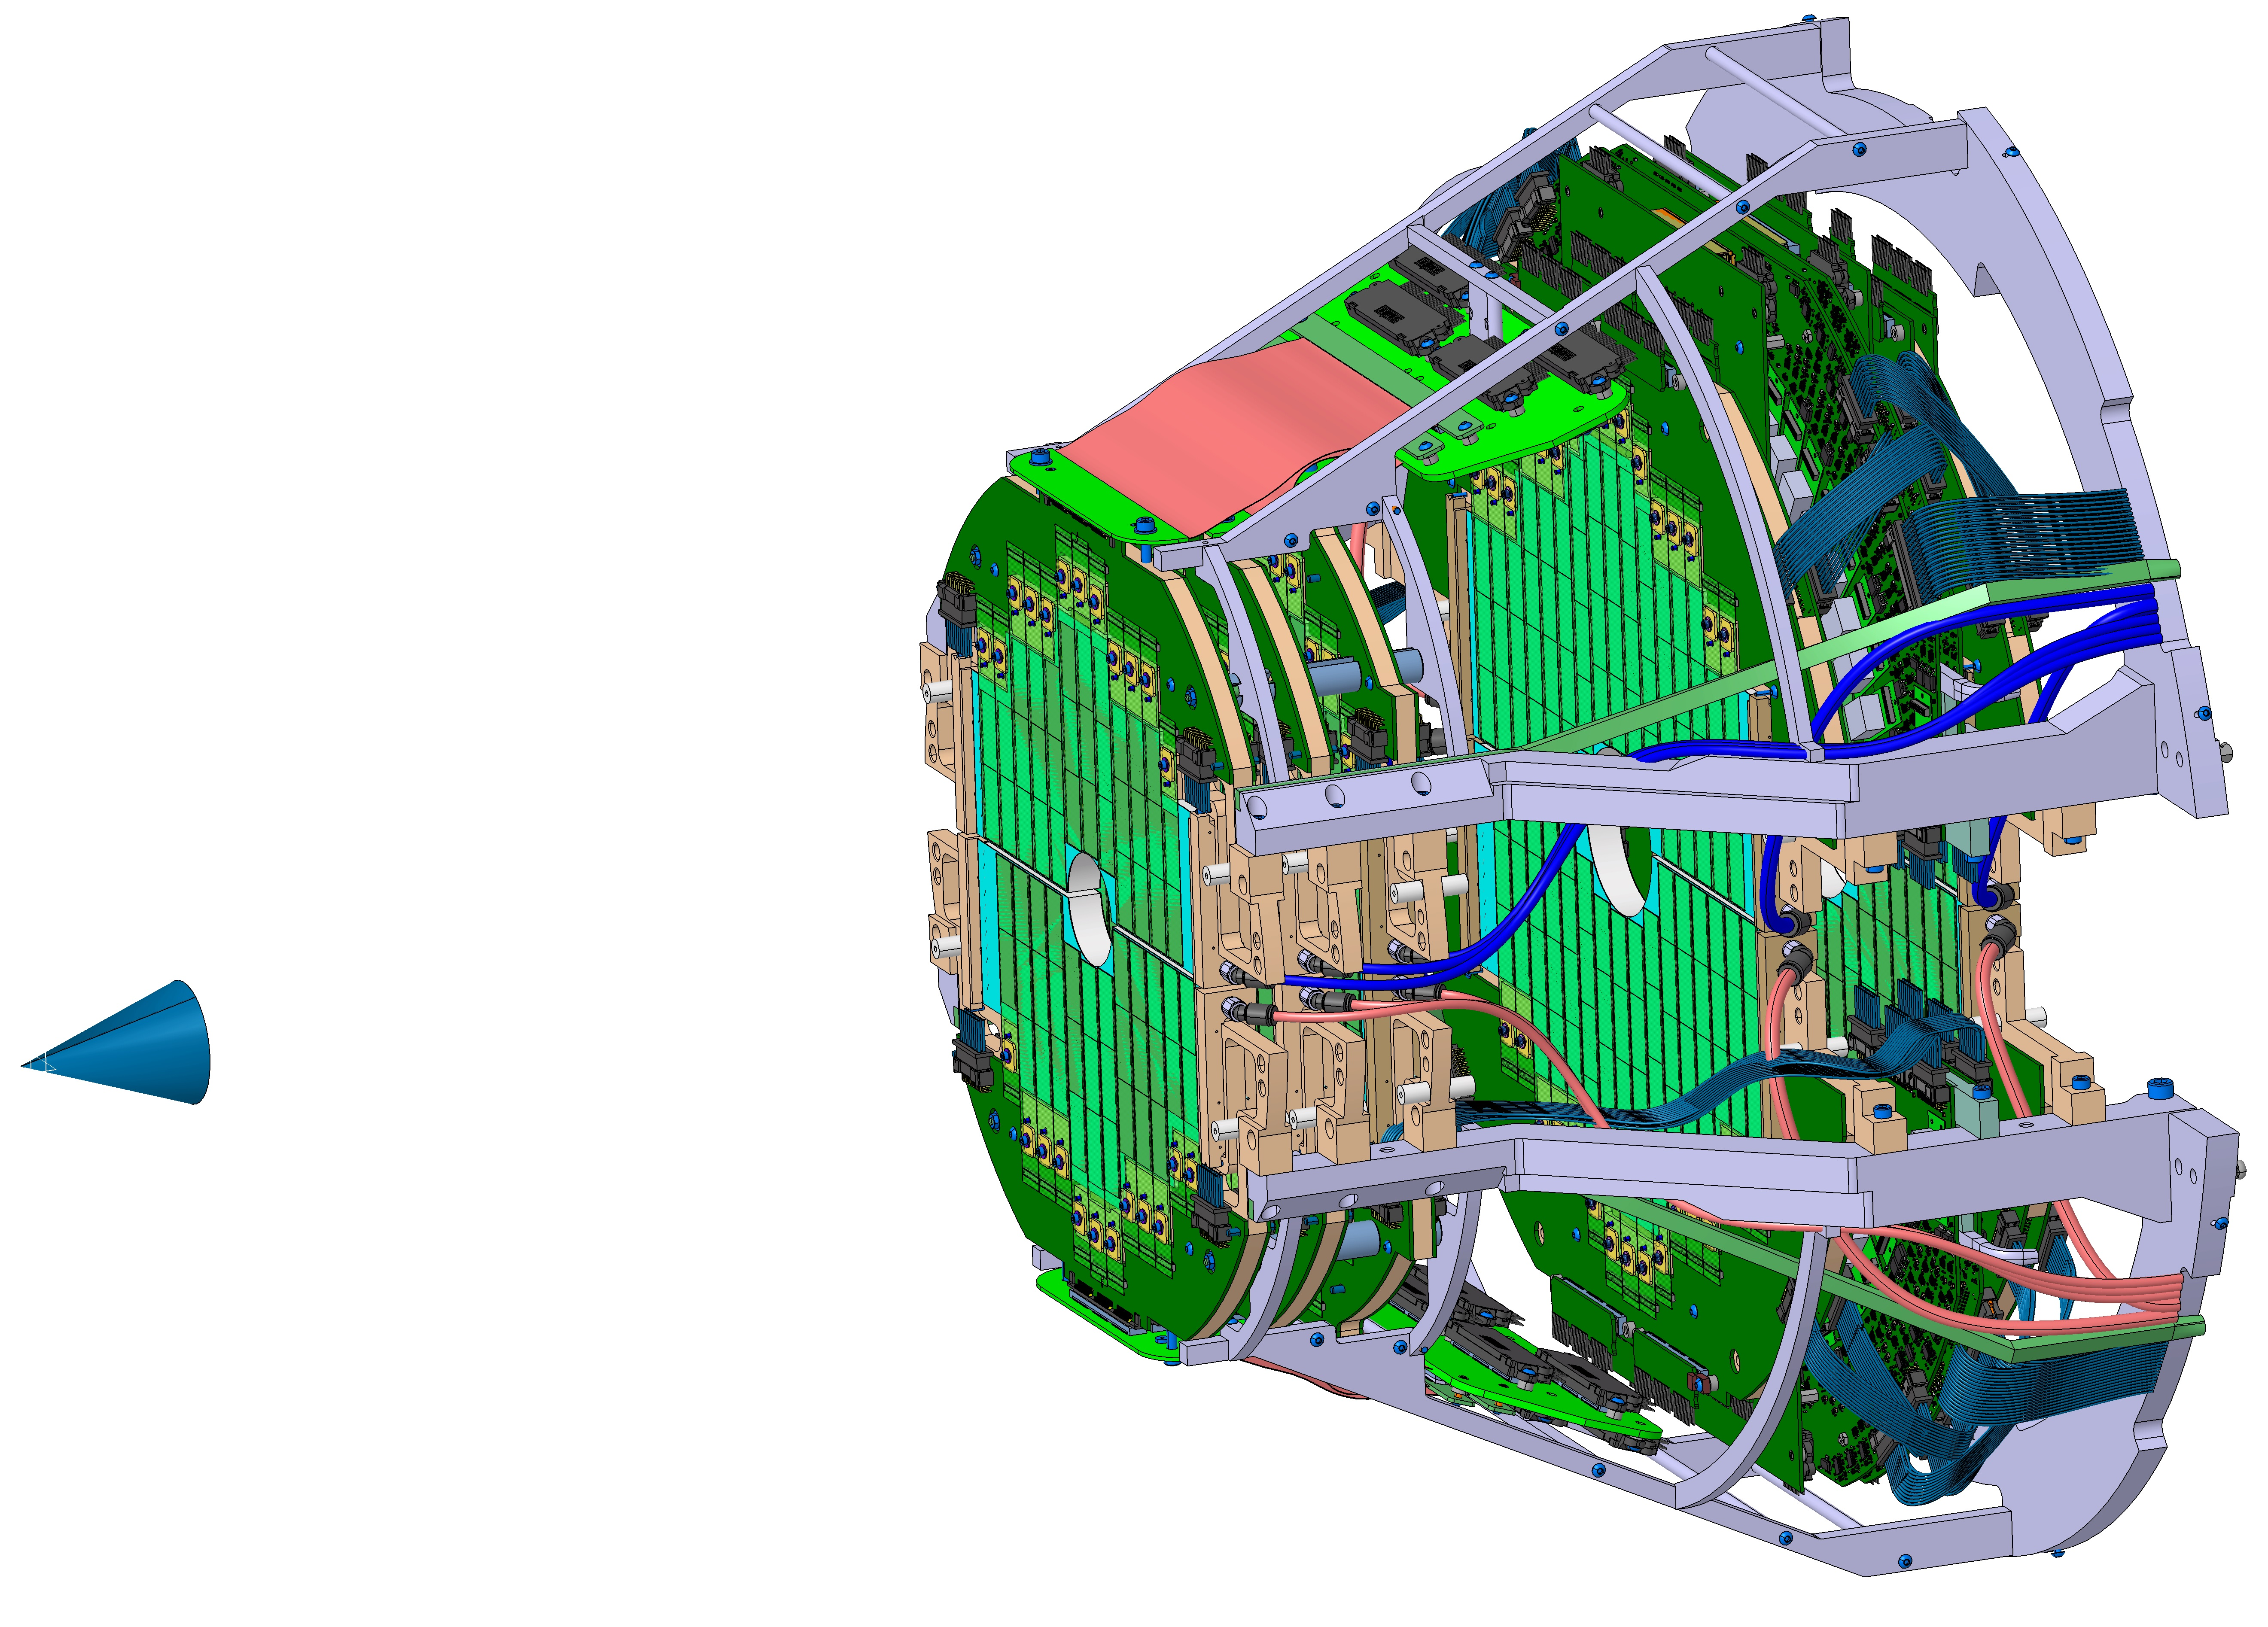
\includegraphics[width=.8\textwidth]{Figs/MFT_schematic.jpg}
        \caption{Schematic view of the Muon Forward Tracker~\cite{MFT_Schematic}. The small cone on the left shows the IP.}
        \label{fig:MFT Schematic}
    \end{center}
\end{figure}

The MFT Technical Design Report \cite{MFT_TDR} gives all the details on the construction and implementation of the MFT, but the points relevant to this report will be discussed here.

The MFT is made up of 5 disks, each made of 2 half-disks. Each half disk has two planes of detectors, one on the front and one on the back. The disks sit at $z$-positions -46.0, -49.3, -53.1, -68.7, and -76.8 \si{\centi\metre} respectively and each disk is \SI{1.4}{\centi\metre} thick, leading to detector planes at $\pm \SI{0.7}{\centi\metre}$ from each of those positions. 


\subsection{The Online-Offline Analysis Framework}
With the increased interaction rate expected for Run 3, a new system for real-time processing, as well as offline analysis, needed to be constructed \cite{ALICE_Upgrade_LOI}. The Online-Offline (O2) framework was developed for this purpose. The ``Online'' portion of the framework is the real-time processing, where continuously captured data from ALICE is split into \SI{10}{\milli\second} chunks, called timeframes. These timeframes are then later processed, or ``reconstructed'' into Analysis Object Data (AOD) files---this is the ``Offline'' part--- which contain only the data of interest. Different passes of reconstruction can be done for purposes. These AOD files can then be analysed, also Offline, through an ``Analysis Task'', written in C\texttt{++} and ROOT. 

We distinguish between data taken in Run 3 and data taken in Run 1 and 2 by calling Run 3 AOD's ``AO2D'' files, and Run 1 and 2 just ``AOD'' files. The data is stored on the \texttt{alimonitor} system, requiring a certificate to access, which is obtained by joining the ALICE collaboration. Access to all data and most analysis tools used in this report is restricted behind this wall. 

\begin{figure}[h]
    \begin{center}
        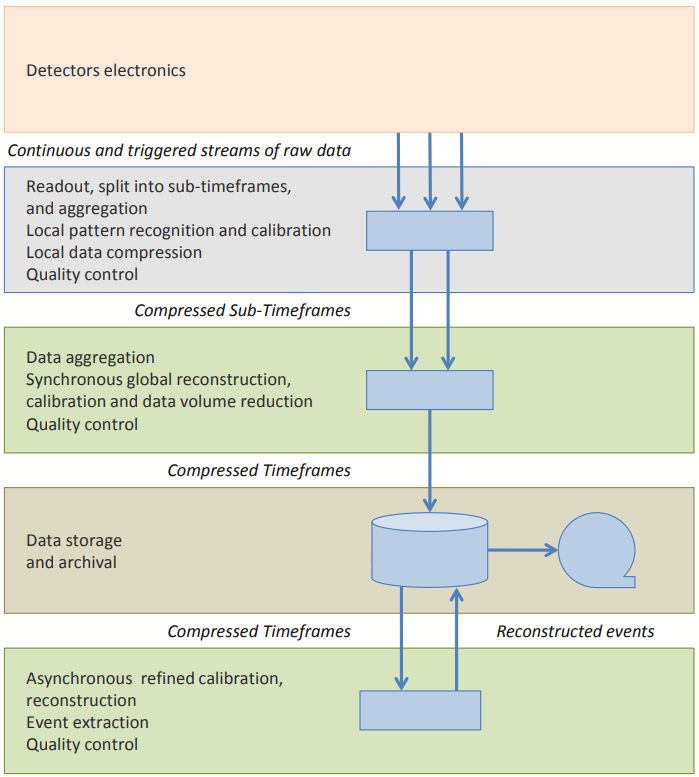
\includegraphics[width=.6\textwidth]{Figs/O2_flow.png}
        \caption{Functional flow of the O2 framework~\cite{O2_Upgrade_TDR}.}
        \label{fig:O2_flow}
    \end{center}
\end{figure}

The focus of the upgraded analysis framework was to reduce disk space usage when processing and analysing, as well as making sure all analysis takes advantage of all processing power available to it at all times. \Cref{fig:O2_flow} shows the general flow of data in the O2 processing pipeline.

